\documentclass[a4paper,12pt]{report}

%\newcommand{\song}{\CJKfamily{song}}  %设置全局字体宋体 12pt = 小四
\usepackage{ctex}
\usepackage{xeCJK}    % CJK 包
\usepackage{times} %英文默认new Roman
\usepackage{setspace}
\usepackage{fancyhdr}
\usepackage{graphicx}
\usepackage{wrapfig}
\usepackage{array}  
\usepackage{fontspec,xunicode,xltxtra}
\usepackage{titlesec}
\usepackage{titletoc}
\usepackage[titletoc]{appendix}
\usepackage[top=30mm,bottom=30mm,left=20mm,right=20mm]{geometry}
\usepackage{cite}
\usepackage{listings}
\usepackage{float}
\usepackage[framed,numbered,autolinebreaks,useliterate]{mcode} % 插入代码
\XeTeXlinebreaklocale "zh"
\XeTeXlinebreakskip = 0pt plus 1pt minus 0.1pt

\setmainfont{Times New Roman}    % 设置西文字体

%---------------------------------------------------------------------
%	页眉页脚设置
%---------------------------------------------------------------------
\fancypagestyle{plain}{
	\pagestyle{fancy}      %改变章节首页页眉
}

\pagestyle{fancy}
\lhead{\kaishu~计算机系统报告~}
\rhead{\kaishu~111111111 魏于翔~}
\cfoot{\thepage}

%---------------------------------------------------------------------
%	章节标题设置
%---------------------------------------------------------------------
\titleformat{\chapter}{\centering\zihao{-1}\heiti}{\thechapter}{1em}{}
\titlespacing{\chapter}{0pt}{*0}{*6}

%---------------------------------------------------------------------
%	摘要标题设置
%---------------------------------------------------------------------
\renewcommand{\abstractname}{\zihao{-3} 摘\quad 要}

%---------------------------------------------------------------------
%	参考文献设置
%---------------------------------------------------------------------
\renewcommand{\bibname}{\zihao{2}{\hspace{\fill}参\hspace{0.5em}考\hspace{0.5em}文\hspace{0.5em}献\hspace{\fill}}}

%---------------------------------------------------------------------
%	引用文献设置为上标
%---------------------------------------------------------------------
\makeatletter
\def\@cite#1#2{\textsuperscript{[{#1\if@tempswa , #2\fi}]}}
\makeatother

%---------------------------------------------------------------------
%	目录页设置
%---------------------------------------------------------------------
\titlecontents{chapter}[0em]{\songti\zihao{-4}}{\thecontentslabel\ }{}
{\hspace{.5em}\titlerule*[4pt]{$\cdot$}\contentspage}
\titlecontents{section}[2em]{\vspace{0.1\baselineskip}\songti\zihao{-4}}{\thecontentslabel\ }{}
{\hspace{.5em}\titlerule*[4pt]{$\cdot$}\contentspage}
\titlecontents{subsection}[4em]{\vspace{0.1\baselineskip}\songti\zihao{-4}}{\thecontentslabel\ }{}
{\hspace{.5em}\titlerule*[4pt]{$\cdot$}\contentspage}


\begin{document}
%---------------------------------------------------------------------
%	封面设置
%---------------------------------------------------------------------
\begin{titlepage}
	\begin{center}
		
    
\includegraphics[width=0.6\textwidth]{figure//HIT.jpg}\\
    \vspace{1cm}
    \textsc{\LARGE Harbin Institute of Technology}\\[1.5cm]
    	
	% 标题
	\hrulefill \\[0.4cm]
	{ \huge \bfseries Y86指令集的SEQ模式CPU设计}\\[0.4cm]
	\hrulefill \\[1.5cm]
	
	\vspace{\fill}
	
\setlength{\extrarowheight}{3mm}

{\songti\zihao{3}	
\begin{tabular}{rl}
	
	%作者信息
	{\makebox[4\ccwd][s]{姓\qquad 名:}}& ~\kaishu 魏\quad 于\quad 翔\\
	
	{\makebox[4\ccwd][s]{学\qquad 号:}}& ~\kaishu 11111111111 \\ 

    {\makebox[4\ccwd][s]{学\qquad 院:}}& ~\kaishu 计算机科学与技术学院\\ 
   	
\end{tabular}
 }\\[2cm]
\vspace{\fill}

{\large \today}% 底部插入当日日期

	\end{center}	

\end{titlepage}

%---------------------------------------------------------------------
%  摘要页
%---------------------------------------------------------------------
\begin{abstract}
\begin{spacing}{1.5}
	{\zihao{-4}
	此处为摘要
	
	此处为摘要\\[0.5cm]
	
	\textbf{关键字}:\quad 摘要 \quad 摘要 \quad 摘要 \quad 摘要
	}
\end{spacing}
\end{abstract}

%---------------------------------------------------------------------
%  目录页
%---------------------------------------------------------------------
\tableofcontents % 生成目录

%---------------------------------------------------------------------
%  实验一
%---------------------------------------------------------------------
\chapter{Y86-64指令集体系结构}
\setcounter{page}{1}
\begin{spacing}{1.5} %行间距?
\songti\zihao{-4}
\section{基本变量}
	CPU中共有15个64位的程序寄存器,指示指令的PC的长度也为64位。CPU还有三个标志位,分别是零标志zf、符号标志sf、溢出标志of,这三个标志位统称为CC。
	
\section{Y86-64指令}
	Y86-64指令集基本上是x86-64指令集的一个自己。它只包括8字节整数操作,寻址方式较少,操作也较少。图1.2中,左边是指令的汇编码,右边是字节编码。可以看出,Y86-64指令每条需要1~10字节不等,这取决于需要哪些字段。每条指令的第一个字节表明指令的类型。这个字节分为两个部分,每部分4位:高4位是代码(code)部分,低4位是功能(function)部分。
	
	我们要实现的CPU还增加了一条指令IADDQ,功能如下图1.3:
	
	\begin{figure}[htb] %若换为H表示固定死图片
		\centering
		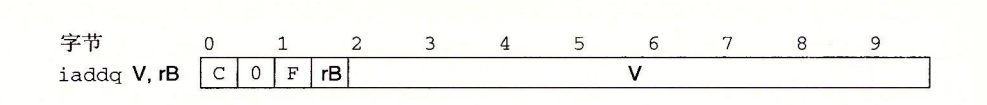
\includegraphics [width=1\textwidth]{figure/IADDQ.png}
		\caption{IADDQ指令}\label{Y86-64}
	\end{figure}

\section{指令编码}

	很多指令都会有一个字节用来表示所用到的寄存器。每个寄存器都用一个数字来表示,使用RNONE(0xF)代表没有用到寄存器。有些指令会有四个字节的立即数,立即数在指令中以小端模式存储。
	
\section{Y86-64异常}

\section{Y86-64程序}
	直接写Y86-64的机器代码,不仅很麻烦,而且容易出错。对日常使用的那些汇编指令集,可以先写汇编代码,然后由汇编器转成机器代码。对于X86-64汇编语言来说,有nasm、masm等汇编器,而对于这里用到的Y86-64汇编语言,也有相应的汇编器yas。通过yas,可以将Y86-64汇编转成机器代码。
	
	下面是一个Y86-64转成机器码的实例:
	
	\begin{lstlisting}
	                            | # Execution begins at address 0 
	0x000:                      | 	.pos 0
	0x000: 30f40002000000000000 | 	irmovq stack, %rsp  # stack pointer
	0x00a: 803800000000000000   | 	call main		# Execute main program
	0x013: 00                   | 	halt			# Terminate program 
	| 
	| # Array of 4 elements
	0x018:                      | 	.align 8
	0x018: 0d000d000d000000     | array:	.quad 0x000d000d000d
	0x020: c000c000c0000000     | 	.quad 0x00c000c000c0
	0x028: 000b000b000b0000     | 	.quad 0x0b000b000b00
	0x030: 00a000a000a00000     | 	.quad 0xa000a000a000
	| 
	0x038: 30f71800000000000000 | main:	irmovq array,%rdi
	0x042: 30f60400000000000000 | 	irmovq $4,%rsi
	0x04c: 805600000000000000   | 	call sum		# sum(array, 4)
	0x055: 90                   | 	ret
	| 
	| # long sum(long *start, long count)
	| # start in %rdi, count in %rsi
	0x056: 30f80800000000000000 | sum:	irmovq $8,%r8        # Constant 8
	0x060: 30f90100000000000000 | 	irmovq $1,%r9	     # Constant 1
	0x06a: 6300                 | 	xorq %rax,%rax	     # sum = 0
	0x06c: 6266                 | 	andq %rsi,%rsi	     # Set CC
	0x06e: 708700000000000000   | 	jmp     test         # Goto test
	0x077: 50a70000000000000000 | loop:	mrmovq (%rdi),%r10   # Get *start
	0x081: 60a0                 | 	addq %r10,%rax       # Add to sum
	0x083: 6087                 | 	addq %r8,%rdi        # start++
	0x085: 6196                 | 	subq %r9,%rsi        # count--.  Set CC
	0x087: 747700000000000000   | test:	jne    loop          # Stop when 0
	0x090: 90                   | 	ret                  # Return
	| 
	| # Stack starts here and grows to lower addresses
	0x200:                      | 	.pos 0x200
	0x200:                      | stack:

	\end{lstlisting}

%\section{一些Y86-64指令的详情}
%	对于pushq的具体执行过程,有两种不同的约定: 1. 压入\%rsp的原始值,2. 压入减去8的\%rsp的值。在我们的CPU中采用的是跟x86-64一样的设计,即压入\%rsp的旧值。
	
%	对于popq也是一样,跟x86-64一样,

\end{spacing}

%---------------------------------------------------------------------
%  实验二
%---------------------------------------------------------------------
\chapter{Y86-64的顺序实现}
\begin{spacing}{1.5}
\section{SEQ}
	SEQ处理器将指令的执行过程分为了六个过程,分别是取指(fetch)、译码(decode)、执行(execute)、访存(memory)、写会(wirte back)、更新PC(PC update)。同时CPU只有一个算数/逻辑单元,根据所执行的指令类型的不同,而进行不同的运算。
	
\section{指令微操作}
	

\section{SEQ硬件结构}


\section{SEQ的时序}

\end{spacing}


%---------------------------------------------------------------------
%  实验二
%---------------------------------------------------------------------
\chapter{SEQ阶段分析和HCL实现}
\begin{spacing}{1.5}
	
\section{取指阶段}	

	
\section{译码和写回阶段}


\section{执行阶段}


\section{访存阶段}
	

\section{更新PC阶段}
	
\end{spacing}



%---------------------------------------------------------------------
%  实验二
%---------------------------------------------------------------------
\chapter{Verilog实现}
\begin{spacing}{1.5}
	
\section{实现过程}

\subsection{顶层模块设计}


\subsection{Fetch阶段设计}

	
\subsection{Decode阶段设计}
	

\subsection{Execute阶段设计}
	

\subsection{Memory阶段设计}
	

\subsection{Write back阶段实现}


\section{结果模拟}
	
\end{spacing}

%---------------------------------------------------------------------
%  实验感想
%---------------------------------------------------------------------
\titleformat{\chapter}{\centering\zihao{-1}\heiti}{}{1em}{}
\chapter{实验总结}
\begin{spacing}{1.5}
	没什么好说的。
\end{spacing}

%---------------------------------------------------------------------
%  参考文献设置
%---------------------------------------------------------------------
\addcontentsline{toc}{chapter}{参考文献}

\begin{thebibliography}{99}
\songti \zihao{-4} 	
	\bibitem{Leslie.{1994}}
	Leslie Lamport. LATEX: A Document Preparation System.AddisonWesley, Reading, Massachusetts, second edition, 1994, ISBN 0-201-52983-1.
	
	\bibitem{Donald.{1984}}
	Donald E. Knuth. The TEXbook, Volume A of Computers and Typesetting,Addison Wesley, Reading, Massachusetts, second edition, 1984,ISBN 0-201-13448-9.Q

	
\end{thebibliography}

%---------------------------------------------------------------------
%  附录设置
%---------------------------------------------------------------------
\titleformat{\chapter}{\heiti\Large}{附录~\Alph{chapter}}{11pt}{\Large}
\titlespacing{\chapter}{0pt}{*-4}{*4}
\lstset{breaklines}                %自动将长的代码行换行排版
\lstset{extendedchars=false}
\lstset{language=Matlab}
\renewcommand{\thechapter}{附录\Alph{chapter}.} 
\appendix
\begin{appendix}
	
\chapter{数据表}
\zihao{-4}\songti
\begin{spacing}{1.5}
	hello world!
\end{spacing}


\chapter{程序代码}
\zihao{-4}\songti
\begin{spacing}{1.5}
下面是一个MATLAB程序的事例,使用了Package mcode,它能较好还原MATLAB本身的编写风格。
\begin{lstlisting}

%代码

\end{lstlisting}
\end{spacing}
\end{appendix}

	

\end{document}
